% Chapter Template

\chapter{LUKS} % Main chapter title

\label{Chapitre 6.1} % Change X to a consecutive number; for referencing this chapter elsewhere, use \ref{ChapterX}

\lhead{ \emph{LUKS}} % Change X to a consecutive number; this is for the header on each page - perhaps a shortened title

%----------------------------------------------------------------------------------------
%	SECTION 1
%----------------------------------------------------------------------------------------


\section{LUKS, cryptsetup, dmcrypt}
\subsection{Installation}

Il faut installer le support dans le noyau avec : 
\begin{lstlisting}[frame=single,style=Console]  % Start your code-block

make linux-menuconfig
\end{lstlisting}

et activer l'option : 
\begin{lstlisting}[frame=single,style=Console]  % Start your code-block

device driver --> Multiple Devices drivers support (RAID and LVM) --> Device mapper support --> Crypt target support
\end{lstlisting}

Et ensuite il faut installer le support dans buildroot avec : 
\begin{lstlisting}[frame=single,style=Console]  % Start your code-block

make menuconfig
\end{lstlisting}

et activer l'option : 
\begin{lstlisting}[frame=single,style=Console]  % Start your code-block

target packages --> hardware handling --> cryptsetup
\end{lstlisting}

Ensuite, après avoir installé le noyau et le rootfs sur la carte SD, on démarre l'Odroid. Pour vérifier si le support à bien été installé on tape la commande : 
\begin{lstlisting}[frame=single,style=Console]  % Start your code-block

cryptsetup --version
\end{lstlisting}

Cryptsetup permet de gérer (lire et écrire) sur des volumes chiffrés par pain dm-crypt et LUKS. Ceci peut s'avérer fort utile lorsque les données utilisateur nécessite un degré de sécurité haut dessus de la normale.
\subsection{Mode plain dm-crypt (plain mode)}
Ce mode permet de chiffrer le périphérique secteur par secteur à l'aide d'une simple clé non-salée ou une passphrase. Aucune vérifications n'est réalisées, et aucune méta données n'est utilisée. De plus, aucune opération de formatage n'est effectuée sur les données. Lorsqu'un périphérique brut est mappé (ouvert), les opérations usuelles peuvent lui être appliquées, incluant la création de système de fichier. Les périphériques ainsi mappés sont généralement disponibles dans \textbf{/dev/mapper/<périphérique>}.
\subsection{Mode LUKS extension mode}
LUKS (Linux Unified Key Setup), est un standard de chiffrement de disque. Il ajoute un entête standardisé au début du périphérique directement suivi d'un espace de clé. Les données chiffrées sont ensuite situées juste après ces deux zones. Le tout forme un "conteneur LUKS". Le périphérique qui possède un conteneur LUKS est communément appelé "LUKS device". Dans la pluspart des cas, les deux nomenclatures peuvent désignés les deux termes. Ã noter que lorsque l'entête LUKS se situe à un offset différent de zéro, le périphérique n'est plus considéré comme un LUKS device mais comme un conteneur LUKS stoqué en mémoire. LUKS peut gérer plusieures passphrases qui peuvent être individuellement révoquées ou changées. Ceci implique un risque lors de l'utilisation de média persistant dû à l'utilisation de  bandes anti-légistes. Les passphrases sont protégées par PBKDF2 contre les attaques de type "bute-force" et dictionaire lequel implémente un hachage et un salage dans la même fonction. Chaque passphrase aussi appelée clé est associée avec l'un des 8 espace-clé. Les opérations clé qui ne sont pas liée à un espace de clé sont affectés au premier espace qui correspond à la passphrase fournie ou au premier espace vide lorsqu'un nouvelle passphrase est fournie.

Pour des raisons de sécurité, le mode "\textbf{LUKS extension}" est recommandé car il bénéficie d'une plus grande sécurité et propose la possibilité d'utiliser 8 clés différentes. Ainsi, l'utilisateur peut chiffrer 8 partitions différentes.

\subsection{Options}
\begin{description}
	\item[--hash, -h] Spécifie le hachage à utiliser lors du hachage du mot de passe. Cette option n'est utilie que lors de l'action de création. La chaîne de hachage est passée à libgcrypt ainsi tout les hashes acceptés par gcrypt sont supportés.
	\item[-key-file, -d] Utilise un fichier comme matériel de clé. Avec LUKS, le matériel de clé fourni par ce fichier via cette option sont toujours utilisés pour les passphrases existantes. Pour créer une nouvelle clé via un fichier de clé, il est nécessaire d'utiliser un argument positionel à luksFormat ou luksAddKey.
	\item[Cipher par défaut] Pour LUKS, le cipher par défaut est "aes-xts-plain64", selon la documentation. \cite{luksCipher}
\end{description}

\subsection{Installation}
Dans cet exercice, la partition \#3 est utilisée comme partition chiffrée. Pour ce faire, il est nécessaire d'installer au préalable le support cryptographique du noyau (\textbf{Crypt target support}). Cette option est sélectionnable dans le menu de configuration du kernel.
\begin{lstlisting}[style=Bash]
make linux-menuconfig
    Device Drivers
[*] Multiple devices driver support (RAID and LVM)
<*>   Device mapper support
<*>     Crypt target support
\end{lstlisting}
Puis installer le packet cryptsetup dans buildroot à l'aide de la commande
\begin{lstlisting}[style=Bash]
make menuconfig
    Target packages  --->
    Hardware handling  --->
[*] cryptsetup
\end{lstlisting}

Puis sur le système embarqué:
\begin{lstlisting}
# cryptsetup --key-size 256 luksFormat /dev/mmcblk0p3

WARNING!
========
This will overwrite data on /dev/mmcblk0p3 irrevocably.

Are you sure? (Type uppercase yes): YES
Enter passphrase: 
Verify passphrase: 
[   75.674159] [c0] bio: create slab <bio-1> at 1
Jan  1 00:01:12 odroidxu3 user.info kernel: [   75.674159] [c0] bio: create slab <bio-1> at 1
[   78.687741] [c5] bio: create slab <bio-1> at 1
Jan  1 00:01:15 odroidxu3 user.info kernel: [   78.687741] [c5] bio: create slab <bio-1> at 1
\end{lstlisting}

\begin{lstlisting}[style=Bash]
# cat 1-emptyLuks.txt 
LUKS header information for /dev/mmcblk0p3

Version:        1
Cipher name:    aes
Cipher mode:    xts-plain64
Hash spec:      sha1
Payload offset: 4096
MK bits:        256
MK digest:      14 d1 64 7b 97 c2 d2 88 8b da a7 8c 9e 40 52 d0 4a ae a9 24 
MK salt:        24 d9 98 89 cd 13 8f 54 4f 59 42 bd 61 fd 47 a3 
                e9 fe 12 52 e5 d4 ef ad 8c 6d f6 86 5e 9c 88 eb 
MK iterations:  24125
UUID:           b2edfb67-b213-4047-bf46-c635ab03b821

Key Slot 0: ENABLED
        Iterations:             99224
        Salt:                   6a 80 7c b0 bf 69 26 0f 61 c2 dd 1a 7b 7d a6 be 
                                90 15 07 fc b3 45 b7 37 08 75 d9 f3 e6 bf a6 d3 
        Key material offset:    8
        AF stripes:             4000
Key Slot 1: DISABLED
Key Slot 2: DISABLED
Key Slot 3: DISABLED
Key Slot 4: DISABLED
Key Slot 5: DISABLED
Key Slot 6: DISABLED
Key Slot 7: DISABLED
# hexdump 1-emptyLuksDump -n 1000
0000000 554c 534b beba 0100 6561 0073 0000 0000
0000010 0000 0000 0000 0000 0000 0000 0000 0000
0000020 0000 0000 0000 0000 7478 2d73 6c70 6961
0000030 366e 0034 0000 0000 0000 0000 0000 0000
0000040 0000 0000 0000 0000 6873 3161 0000 0000
0000050 0000 0000 0000 0000 0000 0000 0000 0000
0000060 0000 0000 0000 0000 0000 0010 0000 2000
0000070 d114 7b64 c297 88d2 da8b 8ca7 409e d052
0000080 ae4a 24a9 d924 8998 13cd 548f 594f bd42
0000090 fd61 a347 fee9 5212 d4e5 adef 6d8c 86f6
00000a0 9c5e eb88 0000 3d5e 3262 6465 6266 3736
00000b0 622d 3132 2d33 3034 3734 622d 3466 2d36
00000c0 3663 3533 6261 3330 3862 3132 0000 0000
00000d0 ac00 f371 0100 9883 806a b07c 69bf 0f26
00000e0 c261 1add 7d7b bea6 1590 fc07 45b3 37b7
00000f0 7508 f3d9 bfe6 d3a6 0000 0800 0000 a00f
0000100 0000 adde 0000 0000 0000 0000 0000 0000
0000110 0000 0000 0000 0000 0000 0000 0000 0000
0000120 0000 0000 0000 0000 0000 0801 0000 a00f
0000130 0000 adde 0000 0000 0000 0000 0000 0000
0000140 0000 0000 0000 0000 0000 0000 0000 0000
0000150 0000 0000 0000 0000 0000 0802 0000 a00f
0000160 0000 adde 0000 0000 0000 0000 0000 0000
0000170 0000 0000 0000 0000 0000 0000 0000 0000
0000180 0000 0000 0000 0000 0000 0803 0000 a00f
0000190 0000 adde 0000 0000 0000 0000 0000 0000
00001a0 0000 0000 0000 0000 0000 0000 0000 0000
00001b0 0000 0000 0000 0000 0000 0804 0000 a00f
00001c0 0000 adde 0000 0000 0000 0000 0000 0000
00001d0 0000 0000 0000 0000 0000 0000 0000 0000
00001e0 0000 0000 0000 0000 0000 0805 0000 a00f
00001f0 0000 adde 0000 0000 0000 0000 0000 0000
0000200 0000 0000 0000 0000 0000 0000 0000 0000
0000210 0000 0000 0000 0000 0000 0806 0000 a00f
0000220 0000 adde 0000 0000 0000 0000 0000 0000
0000230 0000 0000 0000 0000 0000 0000 0000 0000
0000240 0000 0000 0000 0000 0000 0807 0000 a00f
0000250 0000 0000 0000 0000 0000 0000 0000 0000
*
00003e0
\end{lstlisting}

\subsection{Taille de l'en-tête}
l'en-tête de la partition LUKS est représenté par la figure \ref{fig:luks partition header}.
\begin{figure}
	\centering
	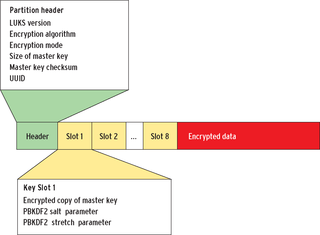
\includegraphics[width=10cm]{q5.6.3/luks-partition-header}
	\caption{\label{fig:luks partition header}En-tête de la partition LUKS}
\end{figure}
Dans ce cas, chaque slot de clé possède 256 bits car la commande utilisée pour créer les clés de partition est la suivante:
\begin{lstlisting}
cryptsetup --verify-passphrase --key-size 256 luksFormat /dev/mmcblk0p3
\end{lstlisting}

Comme la taille de l'en-tête de la partition est inconue, une petite mesure a été réalisée et consiste à ne modifier que la clé maîtresse du chiffrement afin d'en connaître précisément la taille.
\begin{lstlisting}
cryptsetup -y luksAddKey /dev/mmcblk0p3
\end{lstlisting}
http://auto0.info/secret-messages-download-red-hat-fedora

\subsection{Montage sur l'ordinateur hôte}
\begin{lstlisting}
$ sudo mount -t ext4 /dev/mmcblk0p3 /media/embedhfw/usrfs
mount: wrong fs type, bad option, bad superblock on /dev/mmcblk0p3,
       missing codepage or helper program, or other error
       In some cases useful info is found in syslog - try
       dmesg | tail  or so

\end{lstlisting}

\section{Initramfs}
u-boot propose d'utiliser initramfs mais de ce fait, il copie "bêtement" le rootfs là où devrait se trouver initramfs. Ici, l'idée est de faire les choses plus intelligente et générant un initramfs qui sera alors copier sur la \usd. u-boot le chargera ensuite dans la mémoire à l'aide de la commande

Mettre image RAM <-> FLASH

\href{http://forum.odroid.com/viewtopic.php?f=81&t=4860}{}

\subsection{uBoot}
\begin{lstlisting}
set initramfs_addr 0x42000000
set addmmcargs 'setenv bootargs ${bootargs} root=/dev/mmcblk0p2 rw rootwait rootfstype=ext4'
set mmcboot 'run addttyargs addmmcargs addipargs; ext2load mmc 0:1 ${fdts_addr} exynos5422-odroidxu3.dtb; ext2load mmc 0:1 ${kernel_addr} uImage; ext2load mmc 0:1 ${initramfs_addr} uInitrd; bootm ${kernel_addr} ${initramfs_addr} ${fdts_addr}'
saveenv
\end{lstlisting}
Ceci implique que le \textbf{initramfs} doit se trouver à l'adresse \textbf{0x42000000} sur la carte \usd. Celui-là est une image au format cpio archive qui peut être générée manuellement.

Pour installer le support du démarrage du noyau sur initramfs, il est au préalable nécessaire de l'installer à l'aide de buildroot:
\begin{lstlisting}[style=Bash]
make linux-menuconfig
    General setup  --->
[*] Initial RAM filesystem and RAM disk (initramfs/initrd) support
(~/ses/03-labos/labo05/exercice-7/initramfs) Initramfs source file(s)
\end{lstlisting}

\subsection{Contenu}
\begin{lstlisting}
/init
/bin/mount
/lib/libmount.so.1
	/...
\end{lstlisting}

\subsection{Utilité}
Cette technique peut être intéressante lorsqu'il faudrait interfacer un disque IDE avec Linux qui ne possède pas de driver dans le noyau. Ainsi, initramfs possède ce driver et effectue un pre-démarrage du noyau. Dans le fichier /init de initramfs se trouve une ligne permettant le chargement du module IDE (insmod). Ainsi, Linux saura communiquer avec le disque IDE.

Cette technique est largement répandue dans les noyau dit "exotiques" dont celui-ci ne possèderait pas tout les pilotes nativement.

\subsection{Installation dans initramfs}
L'installation de cryptsetup sur la partition initramfs nécessite plusieurs opérations, notamment la copie des librairies dynamiques permettant l'exécution de \textbf{cryptsetup} puis l'installation du module noyau appelé \textbf{dm\_mod}.

\subsubsection{Copie des librairies nécessaires à cryptsetup}
Pour l'installation de cryptsetup dans le système initramfs, il a préalablement été nécessaire d'exécuter la commande strings filtrée sur les librairies afin d'obtenir la liste des dépendances de cryptsetup:
\begin{lstlisting}[style=Bash]
$ strings buildroot/output/target/bin/cryptsetup
/lib/ld-linux-armhf.so.3
libcryptsetup.so.4
libuuid.so.1
libdevmapper.so.1.02
libgcrypt.so.20
libgpg-error.so.0
libpopt.so.0
libc.so.6
\end{lstlisting}
